% Chương 4: Hiện thực hoá hệ thống (bản rút gọn)
\chapter{HIỆN THỰC HOÁ HỆ THỐNG}
\label{chap:hien-thuc}

Chương này mô tả cách kiến trúc ở Chương \ref{chap:kien-truc} được hiện thực thành một hệ thống chạy được, gọi là VNU-Trust. Trọng tâm là những quyết định kỹ thuật có ảnh hưởng tới tính chất an toàn hoặc tới cách đọc kết quả ở Chương \ref{chap:danh-gia}, không phải mô tả đầy đủ mã nguồn. Hệ thống mô phỏng mô hình liên trường của ĐHQGHN; những gì nằm ngoài phạm vi gồm tích hợp hệ thống quản lý đào tạo thật, liên hợp nhiều miền quản trị, mô-đun bảo mật phần cứng cho khoá của cơ quan quản trị và triển khai trên mạng chính.

\section{Môi trường và lựa chọn nền tảng}
\label{sec:moi-truong}

\begin{table}[H]
\centering
\caption{Thành phần và phiên bản của hệ thống thử nghiệm}
\label{tab:v2-env}
\renewcommand{\arraystretch}{1.2}
\small
\begin{tabular}{|p{3.6cm}|p{2.5cm}|p{7.2cm}|}
\hline
\textbf{Thành phần} & \textbf{Phiên bản} & \textbf{Vai trò} \\ \hline
Mạng thử nghiệm Movement & Mã chuỗi 250 & Nguồn sự thật: định danh, thẩm quyền, trạng thái chứng thực \\ \hline
Aptos CLI (biên dịch Move) & 7.11 & Biên dịch, kiểm thử và xuất bản ba mô-đun \\ \hline
TypeScript, Express, \texttt{pg}, \texttt{zod} & 5.7 / 4.21 / 8.13 / 3.24 & Cài đặt thứ nhất của tầng chỉ mục \\ \hline
Go, \texttt{pgx}, \texttt{x/crypto} & 1.23 / 5.7 / 0.31 & Cài đặt thứ hai, thư viện HTTP chuẩn \\ \hline
PostgreSQL & 16 & Chỉ mục dùng chung, nhật ký kiểm toán, kho IPFS mô phỏng \\ \hline
React, Vite, Tailwind & 18.3 / 6.0 / 3.4 & Giao diện theo vai trò \\ \hline
\texttt{@noble/curves}, \texttt{@noble/hashes}, \texttt{@scure/bip39} & 1.9 / 1.8 / 1.6 & Ed25519, SHA3-256, BIP-39 phía máy khách, thay bộ công cụ của nền tảng \\ \hline
Web Cryptography API, IndexedDB & Theo trình duyệt & PBKDF2, AES-256-GCM, lưu bản mã kho khoá \\ \hline
\end{tabular}
\end{table}


Bảng \ref{tab:v2-env} có hai điểm khác một triển khai thông thường. Tầng chỉ mục được viết \emph{hai lần}, bằng TypeScript và bằng Go, trên cùng một hợp đồng giao diện và cùng một lược đồ cơ sở dữ liệu (Mục \ref{sec:hai-cai-dat}). Giao diện \emph{không} dùng bộ công cụ phát triển chính thức của nền tảng chuỗi mà tự ký và gửi giao dịch bằng các thư viện mật mã độc lập (Mục \ref{sec:vi}).

Hệ thống được triển khai trên mạng thử nghiệm công khai Movement, dùng máy ảo Move \cite{Movement2024}. Có bốn lý do. Mô hình hướng tài nguyên của Move \cite{Blackshear2019Move} loại bỏ ở tầng ngôn ngữ việc bản ghi thẩm quyền bị nhân bản hay huỷ ngoài ý muốn. Cơ chế \texttt{friend} cho phép mô-đun thẩm quyền gọi một số hàm nội bộ của mô-đun định danh mà không công khai chúng. Thời gian xác nhận dưới một giây nhờ Block-STM \cite{Gelashvili2023}. Và chỉ trên mạng công khai mới kiểm chứng được yêu cầu N1, tra cứu thẩm quyền không cần tài khoản. Lựa chọn này không mang tính khuyến nghị cho sản xuất: cách giải thích hiện hành của cơ quan bảo vệ dữ liệu nghiêng về chuỗi cấp phép vì trên chuỗi công khai không xác định được ai là bên kiểm soát dữ liệu \cite{EDPB2025}. Đây là lập luận về trách nhiệm pháp lý và nó mạnh hơn lập luận về chi phí. Kiến trúc phân lớp cho phép chuyển sang một chuỗi liên hợp như NDAChain \cite{NDAChain2025} mà không thiết kế lại khung quản trị.

Ba thành phần cùng cần địa chỉ gói hợp đồng và thông số chuỗi: hai cài đặt tầng chỉ mục và giao diện. Ban đầu mỗi thành phần khai riêng trong tệp cấu hình của mình, và khi triển khai lại hợp đồng mà cập nhật sót một tệp, hai cài đặt nói chuyện với hai gói khác nhau mà không thành phần nào báo lỗi. Hiện toàn bộ thông số nằm trong một tệp duy nhất ở gốc dự án, có tập lệnh đồng bộ sang ba nơi, và tập lệnh triển khai tự cập nhật tệp đó sau khi xuất bản. Một giá trị cần nhất quán giữa nhiều thành phần thì phải có đúng một nguồn.

\section{Hợp đồng thông minh}
\label{sec:hop-dong}

\subsection{Ba mô-đun}

\texttt{did\_registry} quản lý định danh và DID Document: đăng ký, cập nhật kèm phiên bản, đình chỉ, kích hoạt lại, thu hồi và phân giải; mô-đun này không phụ thuộc hai mô-đun còn lại. \texttt{authority} quản lý chuỗi thẩm quyền: gốc, quản trị viên, bên phát hành, chuyển quyền gốc hai bước; nó phụ thuộc \texttt{did\_registry} vì một thực thể phải có định danh đang hoạt động mới được cấp thẩm quyền. \texttt{vc\_registry} quản lý bản ghi neo và trạng thái chứng thực; trước khi ghi, nó kiểm thẩm quyền qua \texttt{authority} và trạng thái định danh của cả hai bên qua \texttt{did\_registry}. Quan hệ phụ thuộc là một chiều, đúng nguyên tắc phân lớp.

Trong hàm cấp phát, định danh của bên phát hành \emph{không} lấy từ tham số mà được suy ra từ địa chỉ người ký giao dịch. Nếu lấy từ tham số, một bên phát hành hợp lệ có thể khai định danh của trường khác và tạo ra chứng thực mang tên trường đó, mà mọi phép kiểm chữ ký vẫn đạt.

Bản ghi thẩm quyền, thành phần trung tâm của khung quản trị, có cấu trúc như sau:

\lstinputlisting[language=Move, caption={Cấu trúc bản ghi thẩm quyền trong mô-đun \texttt{authority}}]{source/code/issuer-record.move}

Trường \texttt{vc\_type\_mask} là mặt nạ phạm vi, \texttt{expires\_at} là thời hạn uỷ quyền, hai trường \texttt{delegation\_vc\_*} trỏ tới chứng thực uỷ quyền, còn \texttt{version} hiện thực cơ chế cấp lại mà vẫn giữ dấu vết. Bản ghi định danh có thêm một trường lưu \emph{ai} đã đặt trạng thái đình chỉ. Hệ thống duy trì hai nhóm bộ đếm: tổng số đã từng cấp, chỉ tăng; và số đang hiệu lực, giảm khi thu hồi hay đình chỉ. Nếu chỉ có nhóm đầu, con số ``số văn bằng'' trên giao diện sẽ tính cả văn bằng đã bị thu hồi.

Hợp đồng định nghĩa mã lỗi riêng cho từng loại vi phạm, chia theo ba nhóm ứng với ba mô-đun. Việc này có giá trị trực tiếp cho kiểm thử: một phép kiểm trường hợp vi phạm chỉ có giá trị khi nó thất bại \emph{đúng vì nguyên nhân dự kiến}. Với một mã lỗi chung, không phân biệt được ``phép kiểm thẩm quyền đã chặn'' với ``một phép kiểm định dạng nào đó đã chặn trước''. Trường hợp thứ hai đã thật sự xảy ra: phép kiểm ``mã giao dịch bịa bị từ chối'' cho kết quả đạt, nhưng thực ra là do CID sai định dạng bị chặn trước đó, và bước xác minh giao dịch chưa từng được chạy tới.

\subsection{Mẫu dữ liệu}

Phương thức \texttt{did:vnu} được hiện thực đúng như đặc tả ở Mục \ref{sec:mo-hinh-du-lieu}. Dưới đây là DID Document của một bên phát hành, đúng cấu trúc mà giao diện sinh ra khi đăng ký:

\lstinputlisting[language=json, caption={DID Document của một bên phát hành}]{source/json/issuer-uet.json}

Khoá công khai được biểu diễn ở dạng thập lục phân thay vì đa cơ số, để cùng một giá trị dùng được trực tiếp cho kiểm chữ ký chứng thực và kiểm chữ ký giao dịch. Hai trường \texttt{authentication} và \texttt{assertionMethod} được khai riêng dù trong bản thử nghiệm cùng trỏ tới một khoá; khi tách khoá đăng nhập khỏi khoá cấp phát, điều cần làm trong triển khai thật, cấu trúc tài liệu không phải thay đổi.

Chứng thực văn bằng do bên phát hành sinh ra có dạng:

\lstinputlisting[language=json, caption={Chứng thực văn bằng như giao diện sinh ra}]{source/v2/json/vc.json}

Trường \texttt{expirationDate} chỉ xuất hiện khi văn bằng có thời hạn, và giá trị đó cũng được truyền vào tham số thời hạn của \texttt{issue\_vc}. Có bốn điểm cần nêu rõ, gồm cả những điểm chưa tuân thủ đầy đủ chuẩn. Một là các thuộc tính riêng nằm trong không gian tên \texttt{vnu} khai qua \texttt{@context}, nên một bộ xử lý JSON-LD không nhầm chúng với thuộc tính của chuẩn. Hai là bản thử nghiệm dùng ngữ cảnh của phiên bản 1.1 thay vì 2.0 \cite{W3C_VCDM2025}. Ba là chữ ký được lưu tách rời trong chỉ mục và trong bản trình bày chứ không nhúng trong đối tượng: giá trị băm neo trên chuỗi được tính trên chính đối tượng này, nên nhúng chữ ký vào sẽ phải định nghĩa thêm quy tắc loại trừ trường bằng chứng khi băm. Bốn là không có trường \texttt{credentialStatus} theo danh sách bit; bên xác minh dùng giá trị băm của \texttt{id} làm khoá tra cứu trạng thái trên chuỗi, và kết quả trả về gồm cả trạng thái lẫn giá trị băm nội dung, nên một lần truy vấn phục vụ được cả bước 5 và bước 6. Định danh \texttt{id} là UUID sinh ngẫu nhiên trong trình duyệt; thí nghiệm B ở Chương \ref{chap:danh-gia} cho thấy chính trường này là thứ đang đứng giữa giá trị băm trên chuỗi và một cuộc tấn công từ điển.

\subsection{Rà soát an toàn và xuất bản lại}

Hợp đồng đã qua một đợt rà soát có hệ thống, trong đó mỗi vấn đề được chứng minh bằng một phép kiểm thể hiện hệ quả trước khi sửa. Bảng \ref{tab:v2-audit} tóm tắt mười một vấn đề. Ba trong số đó (V1, V5, V8) không phải lỗi lập trình mà là lỗi mô hình, và chúng đã trở thành ba nguyên tắc thiết kế ở Chương \ref{chap:kien-truc}. Vấn đề V9 thuộc loại khó phát hiện nhất: tham số thời hạn bị ghi cứng bằng không nên toàn bộ nhánh xử lý hết hạn là mã chết, trong khi mã nguồn trông như đã xử lý việc hết hạn. Sau khi sửa, bộ kiểm thử được viết lại theo tiêu chí khác: trước đó mỗi phép kiểm đạt nghĩa là lỗi \emph{có thật}, sau đó nghĩa là lỗi \emph{đã sửa và không quay lại}.

\begin{longtable}{|c|p{5.4cm}|p{7.4cm}|}
\caption{Các vấn đề phát hiện trong đợt rà soát hợp đồng và cách xử lý}
\label{tab:v2-audit} \\
\hline
\textbf{Mã} & \textbf{Vấn đề} & \textbf{Cách xử lý} \\ \hline
\endfirsthead
\hline
\textbf{Mã} & \textbf{Vấn đề} & \textbf{Cách xử lý} \\ \hline
\endhead
V1 & Chuyển quyền gốc một bước & Đề cử rồi ký nhận; hàm khởi tạo tự lấy người xuất bản làm gốc \\ \hline
V2 & Mọi bên phát hành bị đòi băm chứng thực uỷ quyền & Chỉ bắt buộc khi thực sự có quan hệ uỷ quyền \\ \hline
V3 & Không có uỷ quyền nhiều cấp & Thêm với ba ràng buộc ở Mục \ref{sec:uy-quyen} \\ \hline
V4 & Vai trò bị thu hồi không cấp lại được & Cấp lại với phiên bản tăng, giữ bản ghi cũ \\ \hline
V5 & Định danh bị thu hồi khoá địa chỉ vĩnh viễn & Cho đăng ký định danh mới; định danh cũ vẫn tra ra ``đã thu hồi'' \\ \hline
V6 & CID không được kiểm độ dài dù chú thích nói có & Kiểm ở cả ba thao tác ghi CID \\ \hline
V7 & Không phân biệt tự đình chỉ với bị đình chỉ & Thêm trường ghi người đặt trạng thái \\ \hline
V8 & Thu hồi chứng thực đòi thẩm quyền còn hiệu lực & Chỉ cần quyền sở hữu (Mục \ref{sec:bat-doi-xung}) \\ \hline
V9 & Thời hạn chứng thực ghi cứng bằng không, nhánh hết hạn là mã chết & Thời hạn thành tham số thật \\ \hline
V10 & Hàm liệt kê vỡ âm thầm khi vượt giới hạn gas & Thêm hàm phân trang; hàm liệt kê dừng rõ ràng khi vượt ngưỡng \\ \hline
V11 & Nhóm lỗi nhỏ: sai mã lỗi, nhánh chết, số hiệu trùng, xung đột vai trò, bộ đếm & Sửa từng mục \\ \hline
\end{longtable}


Ở bản báo cáo trước, các bản sửa này chỉ tồn tại trong mã nguồn vì gói trên chuỗi vẫn là bản cũ: hàm khởi tạo chỉ chạy một lần, nên muốn đặt lại quản trị viên gốc thì phải xuất bản ở một địa chỉ mới và bỏ lại dữ liệu ở địa chỉ cũ. Gói đã được xuất bản lại tại địa chỉ \texttt{0x0ede7f6b\ldots08e3}, trong đó người xuất bản chính là quản trị viên gốc nhờ bản sửa V1. Bộ đối chiếu tầng chuỗi (Mục \ref{sec:dg-chuc-nang}) xác nhận giao diện chương trình trên chuỗi đã khớp mã nguồn: hàm cấp phát nhận đủ bảy tham số kể cả thời hạn, và hai hàm \texttt{propose\_root}, \texttt{accept\_root} đã tồn tại.

\subsection{Nâng cấp tại chỗ}
\label{sec:nang-cap}

Xuất bản ở địa chỉ mới bỏ lại toàn bộ dữ liệu cũ, nên các sửa đổi sau đó được đưa lên bằng \emph{nâng cấp tại chỗ}: gói được xuất bản với chính sách tương thích, và xuất bản lại cùng địa chỉ, cùng tài khoản là nâng cấp. Chính sách này đặt ba ràng buộc lên mọi thay đổi: không đổi trường của cấu trúc đã có, không đổi hay xoá hàm công khai đã có, và hàm khởi tạo không chạy lại, nên mọi tài nguyên mới phải có một hàm khởi tạo riêng gọi đúng một lần. Gói đã được nâng cấp hai lần. Lần thứ nhất sửa tám vấn đề của đợt rà soát thứ hai, trong đó có việc thu hồi định danh thu hồi luôn vai trò, lan truyền thu hồi theo chuỗi uỷ quyền và việc bên phát hành bị đình chỉ không tự thu hồi được văn bằng của mình nữa, kèm sổ quan hệ uỷ quyền. Lần thứ hai thêm ba chức năng ở Mục \ref{sec:xem-xet}, kèm sổ liên kết thay thế.

Mỗi lần nâng cấp theo cùng một quy trình. Gói được dựng thành tải tin xuất bản rồi gửi tới tuyến mô phỏng với chữ ký toàn số không: nút đầy đủ chạy đủ phép kiểm tương thích mà không ghi gì lên chuỗi. Chỉ khi mô phỏng thành công và người quản lý khoá đồng ý mới gửi thật, rồi gọi hàm khởi tạo tài nguyên mới, cũng sau khi đã mô phỏng. Cuối cùng là ba phép xác minh: số hiệu nâng cấp tăng đúng một, mã nguồn và bản đồ mã nguồn trên chuỗi rỗng, và mã byte của từng mô-đun trên chuỗi trùng khớp giá trị băm SHA-256 với bản dựng cục bộ. Lần nâng cấp thứ hai tốn 3.751 đơn vị gas, đúng bằng con số mô phỏng.

Gói được xuất bản mà \emph{không} kèm mã nguồn. Điều này không giấu được logic: mã byte vẫn công khai và dịch ngược được, còn mã nguồn của lần xuất bản đầu vẫn nằm trong lịch sử giao dịch. Tài khoản xuất bản đồng thời là quản trị viên gốc và giữ quyền nâng cấp mã. Khoá của nó đã được chuyển khỏi thư mục dự án, nhưng vẫn là một khoá duy nhất có thể thay toàn bộ logic của hợp đồng; với triển khai thật, quyền nâng cấp phải thuộc về một ví đa chữ ký, hoặc gói phải được khoá bất biến sau khi ổn định.

\subsection{Xem xét, cấp lại và thu hồi định danh}
\label{sec:xem-xet}

Ba chức năng được thêm ở lần nâng cấp thứ hai giải quyết cùng một câu hỏi: khi có sự cố, bằng chứng trên chuỗi phải thay đổi thế nào mà vẫn giữ được dấu vết.

\textit{Định danh đã thu hồi là vĩnh viễn.} Trước đây một địa chỉ bị thu hồi định danh có thể đăng ký một định danh mới. Vai trò không sống lại, nhưng người bị thu hồi vì gian lận vẫn tự tái lập được danh tính trên đúng địa chỉ cũ mà không qua thủ tục nào. Nay hàm đăng ký từ chối với một mã lỗi riêng; lối thoát cho người dùng chính đáng là ví mới cộng quy trình cấp lại.

\textit{Xem xét theo lô.} Như đã nêu ở Mục \ref{sec:uy-quyen}, thu hồi một đơn vị không vô hiệu hoá văn bằng họ đã cấp. Bốn hàm mới cho quản trị viên và bên uỷ quyền đình chỉ hoặc thu hồi tới 100 văn bằng trong một giao dịch. Mỗi văn bằng đổi trạng thái phát một sự kiện riêng, và một sự kiện tổng kết liệt kê mục nào đã đổi, mục nào bị bỏ qua. Tầng dịch vụ ghi chỉ mục theo \emph{chính sự kiện này} chứ không theo danh sách máy khách gửi lên. Danh sách mã phải tăng dần nghiêm ngặt, một ràng buộc vừa chặn trùng lặp vừa không tốn chi phí bậc hai.

\textit{Cấp lại có liên kết.} Hàm cấp lại, trong \emph{một} giao dịch, cấp văn bằng mới, thu hồi văn bằng cũ với lý do cố định ``replaced'', và ghi liên kết hai chiều cũ--mới vào một sổ riêng; bên xác minh văn bằng cũ thấy ``đã được thay bằng'' cùng mã văn bằng mới. Chỉ bên đã cấp hoặc bên uỷ quyền của họ được cấp lại, và chỉ với văn bằng đang hiệu lực: nếu cho cấp lại một văn bằng đang bị quản trị viên đình chỉ, bên phát hành sẽ làm nhẹ đi quyết định đó bằng một liên kết ``đã thay thế''. Trường hợp ấy, cũng như trường hợp bên đã cấp đã mất thẩm quyền, do quản trị viên nối liên kết. Đổi người nhận sang một ví khác chỉ được phép khi định danh của ví cũ không còn hoạt động, để một bên phát hành không thể chuyển văn bằng của một người đang dùng ví sang người khác. Liên kết \emph{danh tính} giữa ví cũ và ví mới của cùng một người thì không ghi lên chuỗi, vì đó là một mối nối công khai vĩnh viễn giữa hai ví, tức là thông tin cá nhân; nó chỉ nằm trong chỉ mục và nhật ký kiểm toán.

Hai mươi lăm rào chắn mới trong ba chức năng này đều được kiểm bằng kiểm thử đột biến: mỗi rào bị gỡ hoặc làm yếu trên một bản sao của gói, và phải có ít nhất một phép kiểm chuyển sang thất bại. Lần chạy đầu có một rào ``sống sót'': phép kiểm của nó đạt vì một rào khác chặn trước, đúng loại lỗi đã gặp với phép kiểm mã giao dịch bịa. Phép kiểm đã được viết lại để chỉ rào đó chặn được.

\section{Tầng chỉ mục với hai cài đặt độc lập}
\label{sec:hai-cai-dat}

\subsection{Mục đích của cài đặt thứ hai}

Hai cài đặt dùng chung cơ sở dữ liệu và khoá ký phiên, nên phiên đăng nhập do bên này cấp dùng được ở bên kia, và giao diện đổi cài đặt ngay lúc chạy. Mục đích không phải dự phòng mà là biến đặc tả giao diện từ một tài liệu thành một tính chất kiểm chứng được. Khi chỉ có một cài đặt, không phân biệt được một hành vi là quyết định thiết kế hay hệ quả tình cờ của thư viện. Bộ đối chiếu giữa hai cài đặt đã phát hiện ba loại lệch mà kiểm thử thông thường không bắt được. Thứ nhất, thư viện kiểm lược đồ bên TypeScript mặc định \emph{bỏ qua} trường lạ trong thân yêu cầu còn bộ giải mã JSON của Go \emph{từ chối}; cùng một yêu cầu cho hai mã trạng thái khác nhau. Hai bên được thống nhất theo hướng nghiêm ngặt, vì gõ nhầm tên trường thời hạn phải báo lỗi ngay chứ không được âm thầm cấp một văn bằng vô thời hạn. Thứ hai, hai bên kiểm đầu vào theo thứ tự khác nhau nên cùng một yêu cầu sai cho hai mã lỗi khác nhau; hiện cả hai theo thứ tự rẻ trước, đắt sau. Thứ tự kiểm tra đầu vào cũng là một phần của hợp đồng giao diện. Thứ ba, hai tuyến chỉ tồn tại ở bản TypeScript mà bộ đối chiếu vẫn báo đạt trong thời gian dài, vì không phép đối chiếu nào chạm tới chúng.

Ba bất biến phải giống nhau từng byte ở hai cài đặt và ở giao diện, mỗi bất biến có bộ kiểm riêng: chuỗi được ký khi đăng nhập theo cơ chế thách thức -- đáp ứng (lệch một ký tự là chữ ký không bao giờ khớp); phép tuần tự hoá tất định; và hàm băm SHA3-256 trả về tiền tố \texttt{0x} cùng 64 ký tự thập lục phân. Ba nơi dùng ba thư viện khác nhau và đã được đối chiếu cho cùng kết quả, kể cả với ký tự tiếng Việt và cấu trúc lồng sâu.

\subsection{Xác minh giao dịch trước khi ghi chỉ mục}

Theo nguyên tắc ``chỉ mục không phải nguồn sự thật'', mọi bản ghi có tham chiếu trên chuỗi đều mang một mã giao dịch, và tầng dịch vụ kiểm bốn điều với nút đầy đủ trước khi ghi: giao dịch tồn tại, thành công, gọi đúng hàm mong đợi của tuyến, và người gửi khớp tài khoản đang thực hiện yêu cầu. Phép kiểm thứ ba khiến tên hàm hợp đồng xuất hiện ở ba nơi: mã Move, hai cài đặt tầng chỉ mục và tầng chuỗi của giao diện. Sai lệch giữa các nơi này tạo ra kiểu hỏng khó chẩn đoán nhất: giao dịch lên chuỗi thành công nhưng dịch vụ từ chối ghi chỉ mục. Một bộ kiểm đọc trực tiếp mã Move, rút tập hàm công khai và đối chiếu với tên từng thành phần đang dùng. Khi được mở rộng sang nơi gọi thứ ba, bộ kiểm này phát hiện ngay giao diện gọi thao tác đình chỉ chứng thực bằng một tên khác với tên tầng dịch vụ dùng để xác minh.

\subsection{Chế độ không phụ thuộc chuỗi}

Hệ thống có cờ \texttt{VERIFY\_ONCHAIN} để chạy và kiểm thử khi chưa có chuỗi. Phiên bản đầu của cờ chỉ bỏ qua bước xác minh giao dịch mà không bỏ qua việc kiểm quyền trên chuỗi, nên hệ thống vẫn không chạy được khi thiếu chuỗi. Hiện cờ áp dụng nhất quán: khi tắt, cả hai cài đặt bỏ qua xác minh giao dịch \emph{và} trả lời câu hỏi về quyền, định danh, trạng thái bằng chỉ mục cơ sở dữ liệu. Chế độ này không trả lời ``chấp nhận'' vô điều kiện: người học vẫn bị chặn khỏi tuyến của bên phát hành. Nếu không, mọi bộ kiểm thử chạy ở chế độ này chỉ chứng minh rằng hệ thống không báo lỗi. Bốn rào chắn đi kèm: khởi động ở môi trường sản xuất với cờ tắt thì tiến trình thoát ngay; tuyến kiểm tra trạng thái trả giá trị cờ để giao diện hiện dải cảnh báo; mỗi phản hồi báo đúng nguồn dữ liệu là chỉ mục chứ không khai là chuỗi; và một bộ kiểm riêng chứng minh chế độ nghiêm ngặt vẫn chặn mã giao dịch bịa.

Cần lưu ý rằng ở chế độ này, câu hỏi ``trạng thái của chứng thực số hiệu $n$'' được trả lời bằng một truy vấn trên cột \texttt{on\_chain\_vc\_id}, cột không có chỉ mục trong lược đồ. Với dữ liệu thử nghiệm vài trăm bản ghi, điều này không gây ra khác biệt nào đo được; Mục \ref{sec:tn-scale} cho thấy hệ quả khi dữ liệu tăng hai bậc.

\subsection{Chống phát lại và số lần truy vấn chuỗi}

Bốn điều kiện ở mục trước chứng minh một giao dịch có thật, nhưng không chứng minh nó \emph{còn đúng}. Một giao dịch đình chỉ văn bằng có thật, gửi lại sau khi quản trị viên đã kích hoạt văn bằng lại, qua được cả bốn phép kiểm và làm chỉ mục nói sai trạng thái. Vì vậy mọi tuyến đổi trạng thái, sau khi xác minh giao dịch, còn hỏi lại chuỗi trạng thái \emph{hiện tại} và chỉ ghi khi nó đúng là trạng thái sắp ghi. Cũng theo nguyên tắc chỉ mục không phải nguồn sự thật, mọi tuyến quản trị, kể cả tuyến chỉ đọc nhật ký hay số liệu, đối chiếu quyền quản trị trên chuỗi chứ không chỉ đọc vai trò trong cơ sở dữ liệu, để người bị thu hồi quyền từ ngoài ứng dụng không đọc tiếp được dữ liệu của người khác.

Cái giá của nguyên tắc này là số lần gọi tới nút đầy đủ. Đếm trên một nút đầy đủ giả lập cho thấy danh sách hai mươi văn bằng của một chủ thể tốn hai mươi lần gọi, một lần xác minh tám văn bằng tốn hai mươi lăm lần. Hai thay đổi đưa các con số đó về một và ba. Một là đọc trạng thái theo lô bằng hàm phân trang có sẵn trên chuỗi: bản ghi trả về đã mang trạng thái hiệu lực và giá trị băm nội dung, nên thay được cả phép tra trạng thái lẫn phép đối chiếu toàn vẹn. Hai là chỉ hỏi thẩm quyền của mỗi bên phát hành một lần. Phép kiểm quyền quản trị ở mỗi yêu cầu được đệm năm giây theo địa chỉ. Cửa sổ rủi ro được ghi rõ: người vừa bị thu hồi quyền còn đọc được tuyến quản trị tối đa năm giây, nhưng mọi thao tác ghi vẫn bị hợp đồng từ chối, và phép hỏi lại trạng thái chống phát lại không bao giờ được đệm. Kết quả đo ở Mục \ref{sec:truy-van-chuoi}.

Cả hai cài đặt ghi nhật ký kiểm toán với cùng bộ tên hành động. Bảng nhật ký từng nằm sẵn trong lược đồ từ đầu mà \emph{không cài đặt nào ghi vào}, nên tuyến đọc nhật ký luôn trả về rỗng, và không bộ kiểm thử nào phát hiện vì chúng chỉ kiểm định dạng phản hồi. Một bảng có trong lược đồ không có nghĩa là có ai ghi vào nó.

\section{Ví định danh và tầng chuỗi phía máy khách}
\label{sec:vi}

\subsection{Bảo vệ khoá và khôi phục}

Khoá riêng Ed25519 được sinh trong trình duyệt, mã hoá bằng AES-256-GCM với khoá dẫn xuất qua PBKDF2-SHA256 600.000 vòng và muối 16 byte riêng cho mỗi ví; chỉ bản mã nằm trong IndexedDB (Hình \ref{fig:v2-wallet}). Khoá dạng rõ chỉ tồn tại trong bộ nhớ phiên và ví tự khoá sau 15 phút. Đăng nhập là ký một số dùng một lần, nên không mật khẩu nào đi qua mạng. Tầng dịch vụ chỉ giữ bản ghi công khai của mỗi thực thể (địa chỉ, khoá công khai, định danh, vai trò): đó là một cuốn danh bạ, không phải kho tài khoản. Biết địa chỉ của một người mà không có khoá riêng thì không đăng nhập được. Đánh đổi đã chấp nhận và được cảnh báo rõ trên giao diện: mất mật khẩu là mất ví.

\begin{figure}[H]
    \centering
    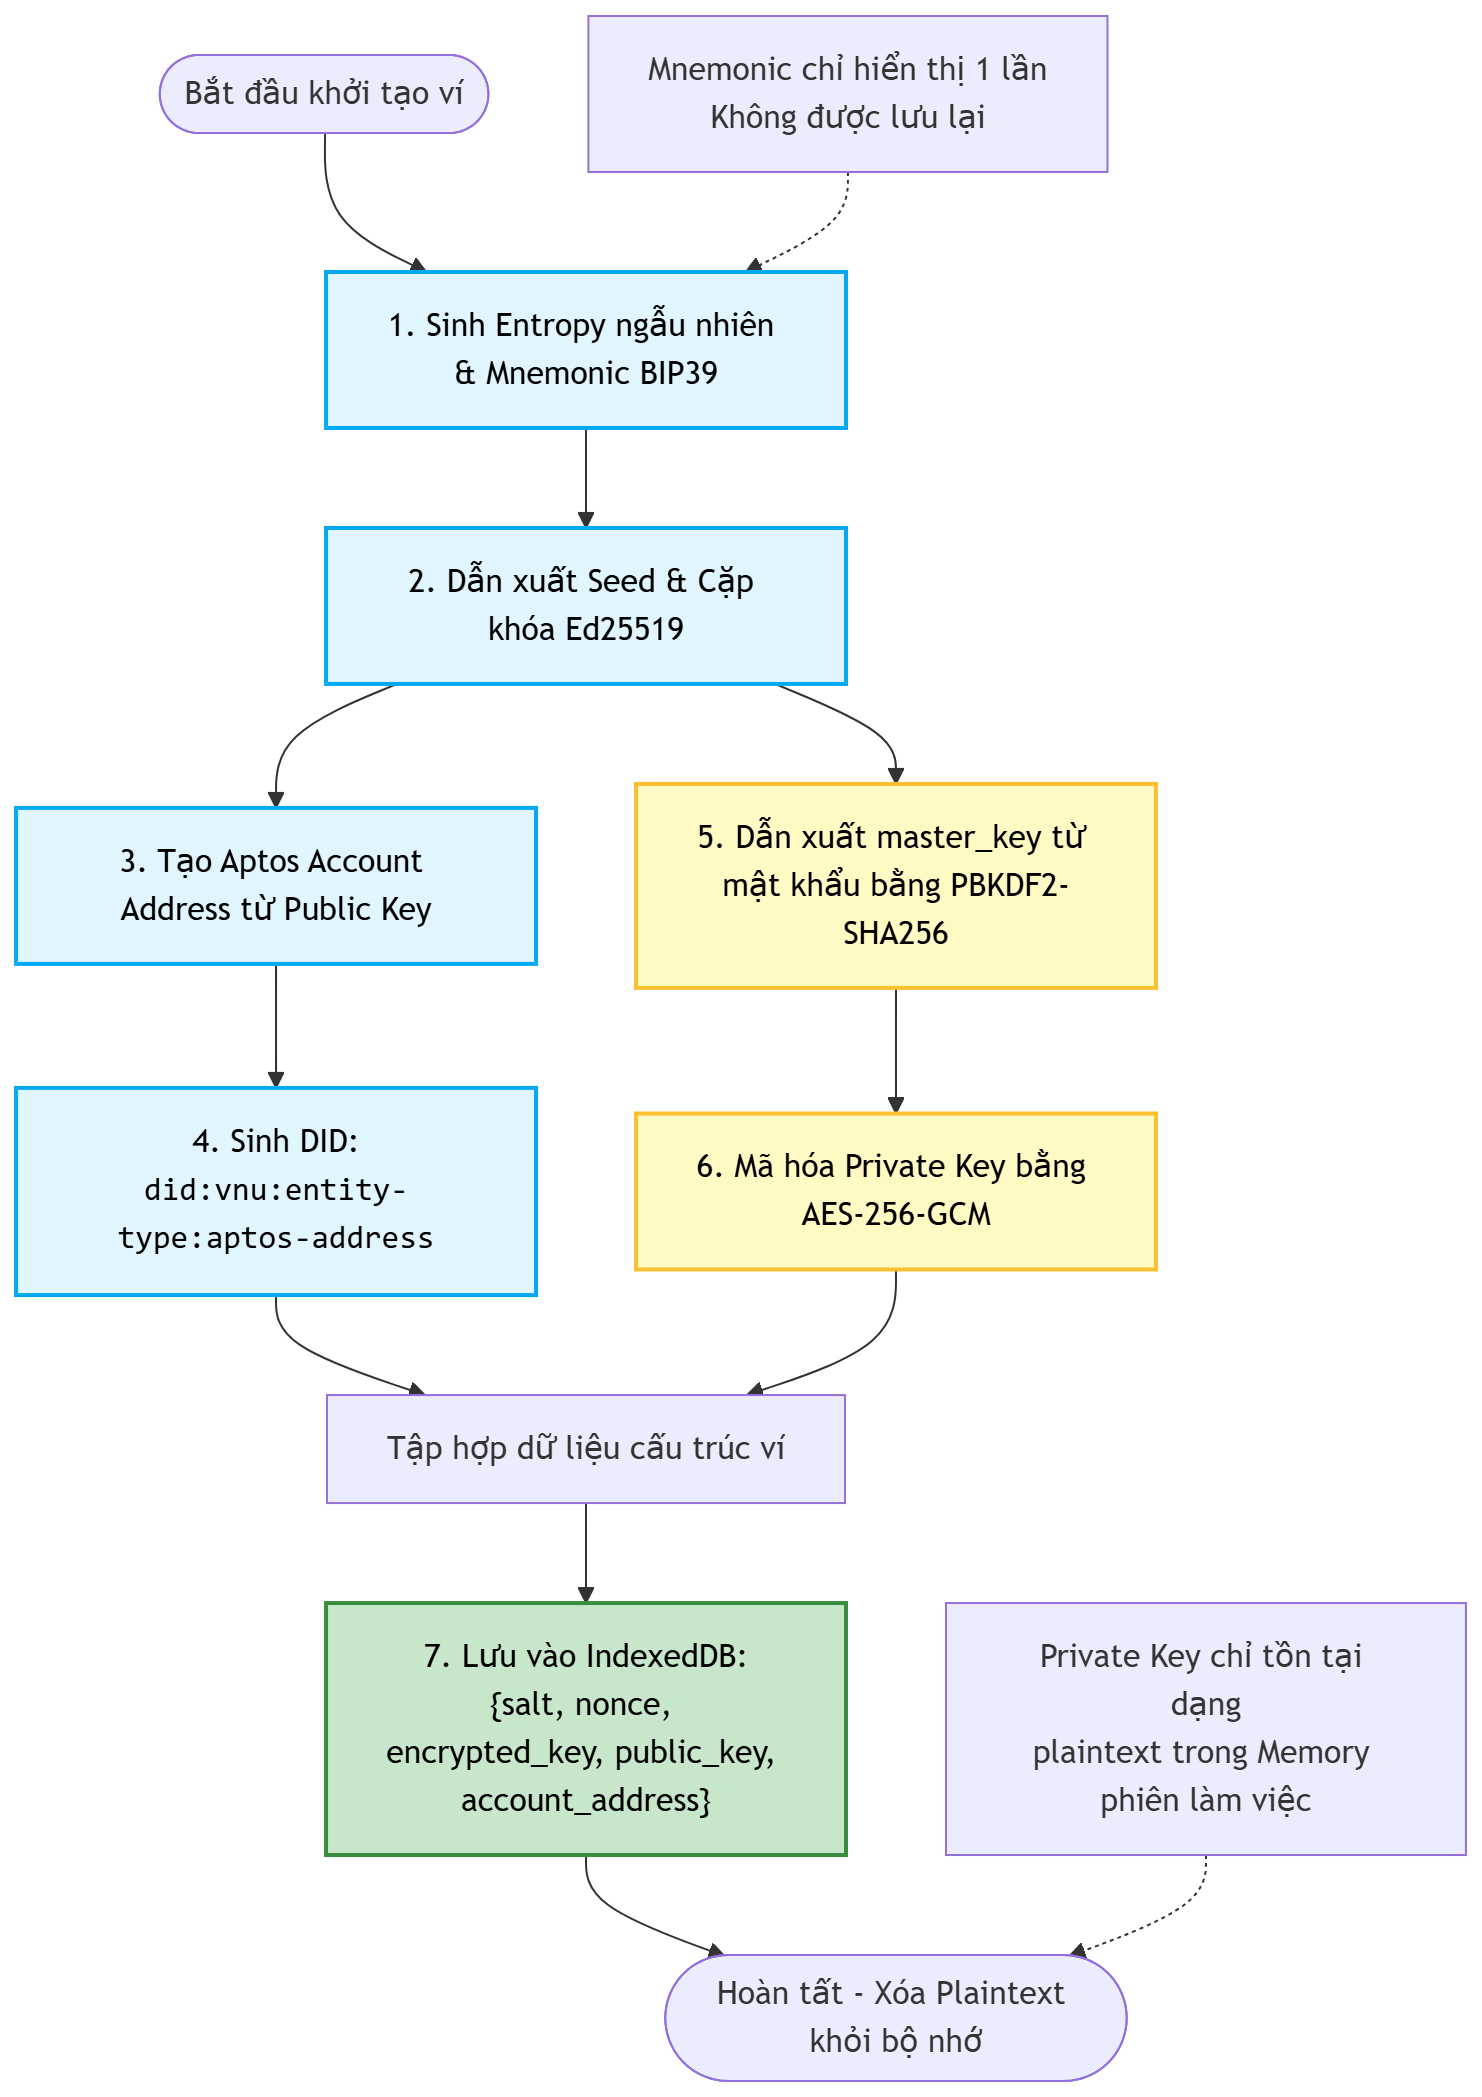
\includegraphics[width=0.42\textwidth]{images/khoi-tao-vi.png}
    \caption{Các bước sinh khoá và lưu trữ khi khởi tạo ví}
    \label{fig:v2-wallet}
\end{figure}

Bảng \ref{tab:v2-wallet} tóm tắt các lớp bảo vệ. Hình \ref{fig:v2-unlock} là trình tự khi người dùng quay lại mở ví để đăng nhập hoặc dựng bản trình bày: mật khẩu chỉ dùng để dẫn xuất khoá giải mã ngay trong trình duyệt, khoá riêng được giải mã vào bộ nhớ phiên, và tầng dịch vụ chỉ nhận chữ ký.

\begin{table}[H]
\centering
\caption{Mô hình bảo vệ khoá của ví không lưu ký}
\label{tab:v2-wallet}
\renewcommand{\arraystretch}{1.2}
\small
\begin{tabular}{|p{3.2cm}|p{10.2cm}|}
\hline
\textbf{Lớp bảo vệ} & \textbf{Cách thực hiện} \\ \hline
Sinh khoá & Ed25519 từ cụm 12 từ BIP-39 sinh bằng nguồn ngẫu nhiên mật mã của trình duyệt \\ \hline
Lưu trữ & Chỉ bản mã nằm trong IndexedDB của thiết bị; khoá dạng rõ không bao giờ được ghi xuống \\ \hline
Mã hoá & AES-256-GCM, khoá dẫn xuất bằng PBKDF2-HMAC-SHA256 600.000 vòng, muối 16 byte riêng mỗi ví \\ \hline
Mật khẩu & Ít nhất 10 ký tự, ít nhất ba trong bốn loại ký tự \\ \hline
Thời gian trong bộ nhớ & Khoá dạng rõ chỉ tồn tại khi ví mở; tự khoá sau 15 phút không thao tác \\ \hline
Đăng nhập & Thách thức -- đáp ứng với số dùng một lần; không mật khẩu nào qua mạng \\ \hline
Sao lưu & Tệp kho khoá xuất ra vẫn ở dạng đã mã hoá \\ \hline
Dữ liệu dịch vụ giữ & Địa chỉ, khoá công khai, định danh, vai trò, nhãn; không băm mật khẩu, không khoá riêng, không cụm từ \\ \hline
\end{tabular}
\end{table}


\begin{figure}[H]
    \centering
    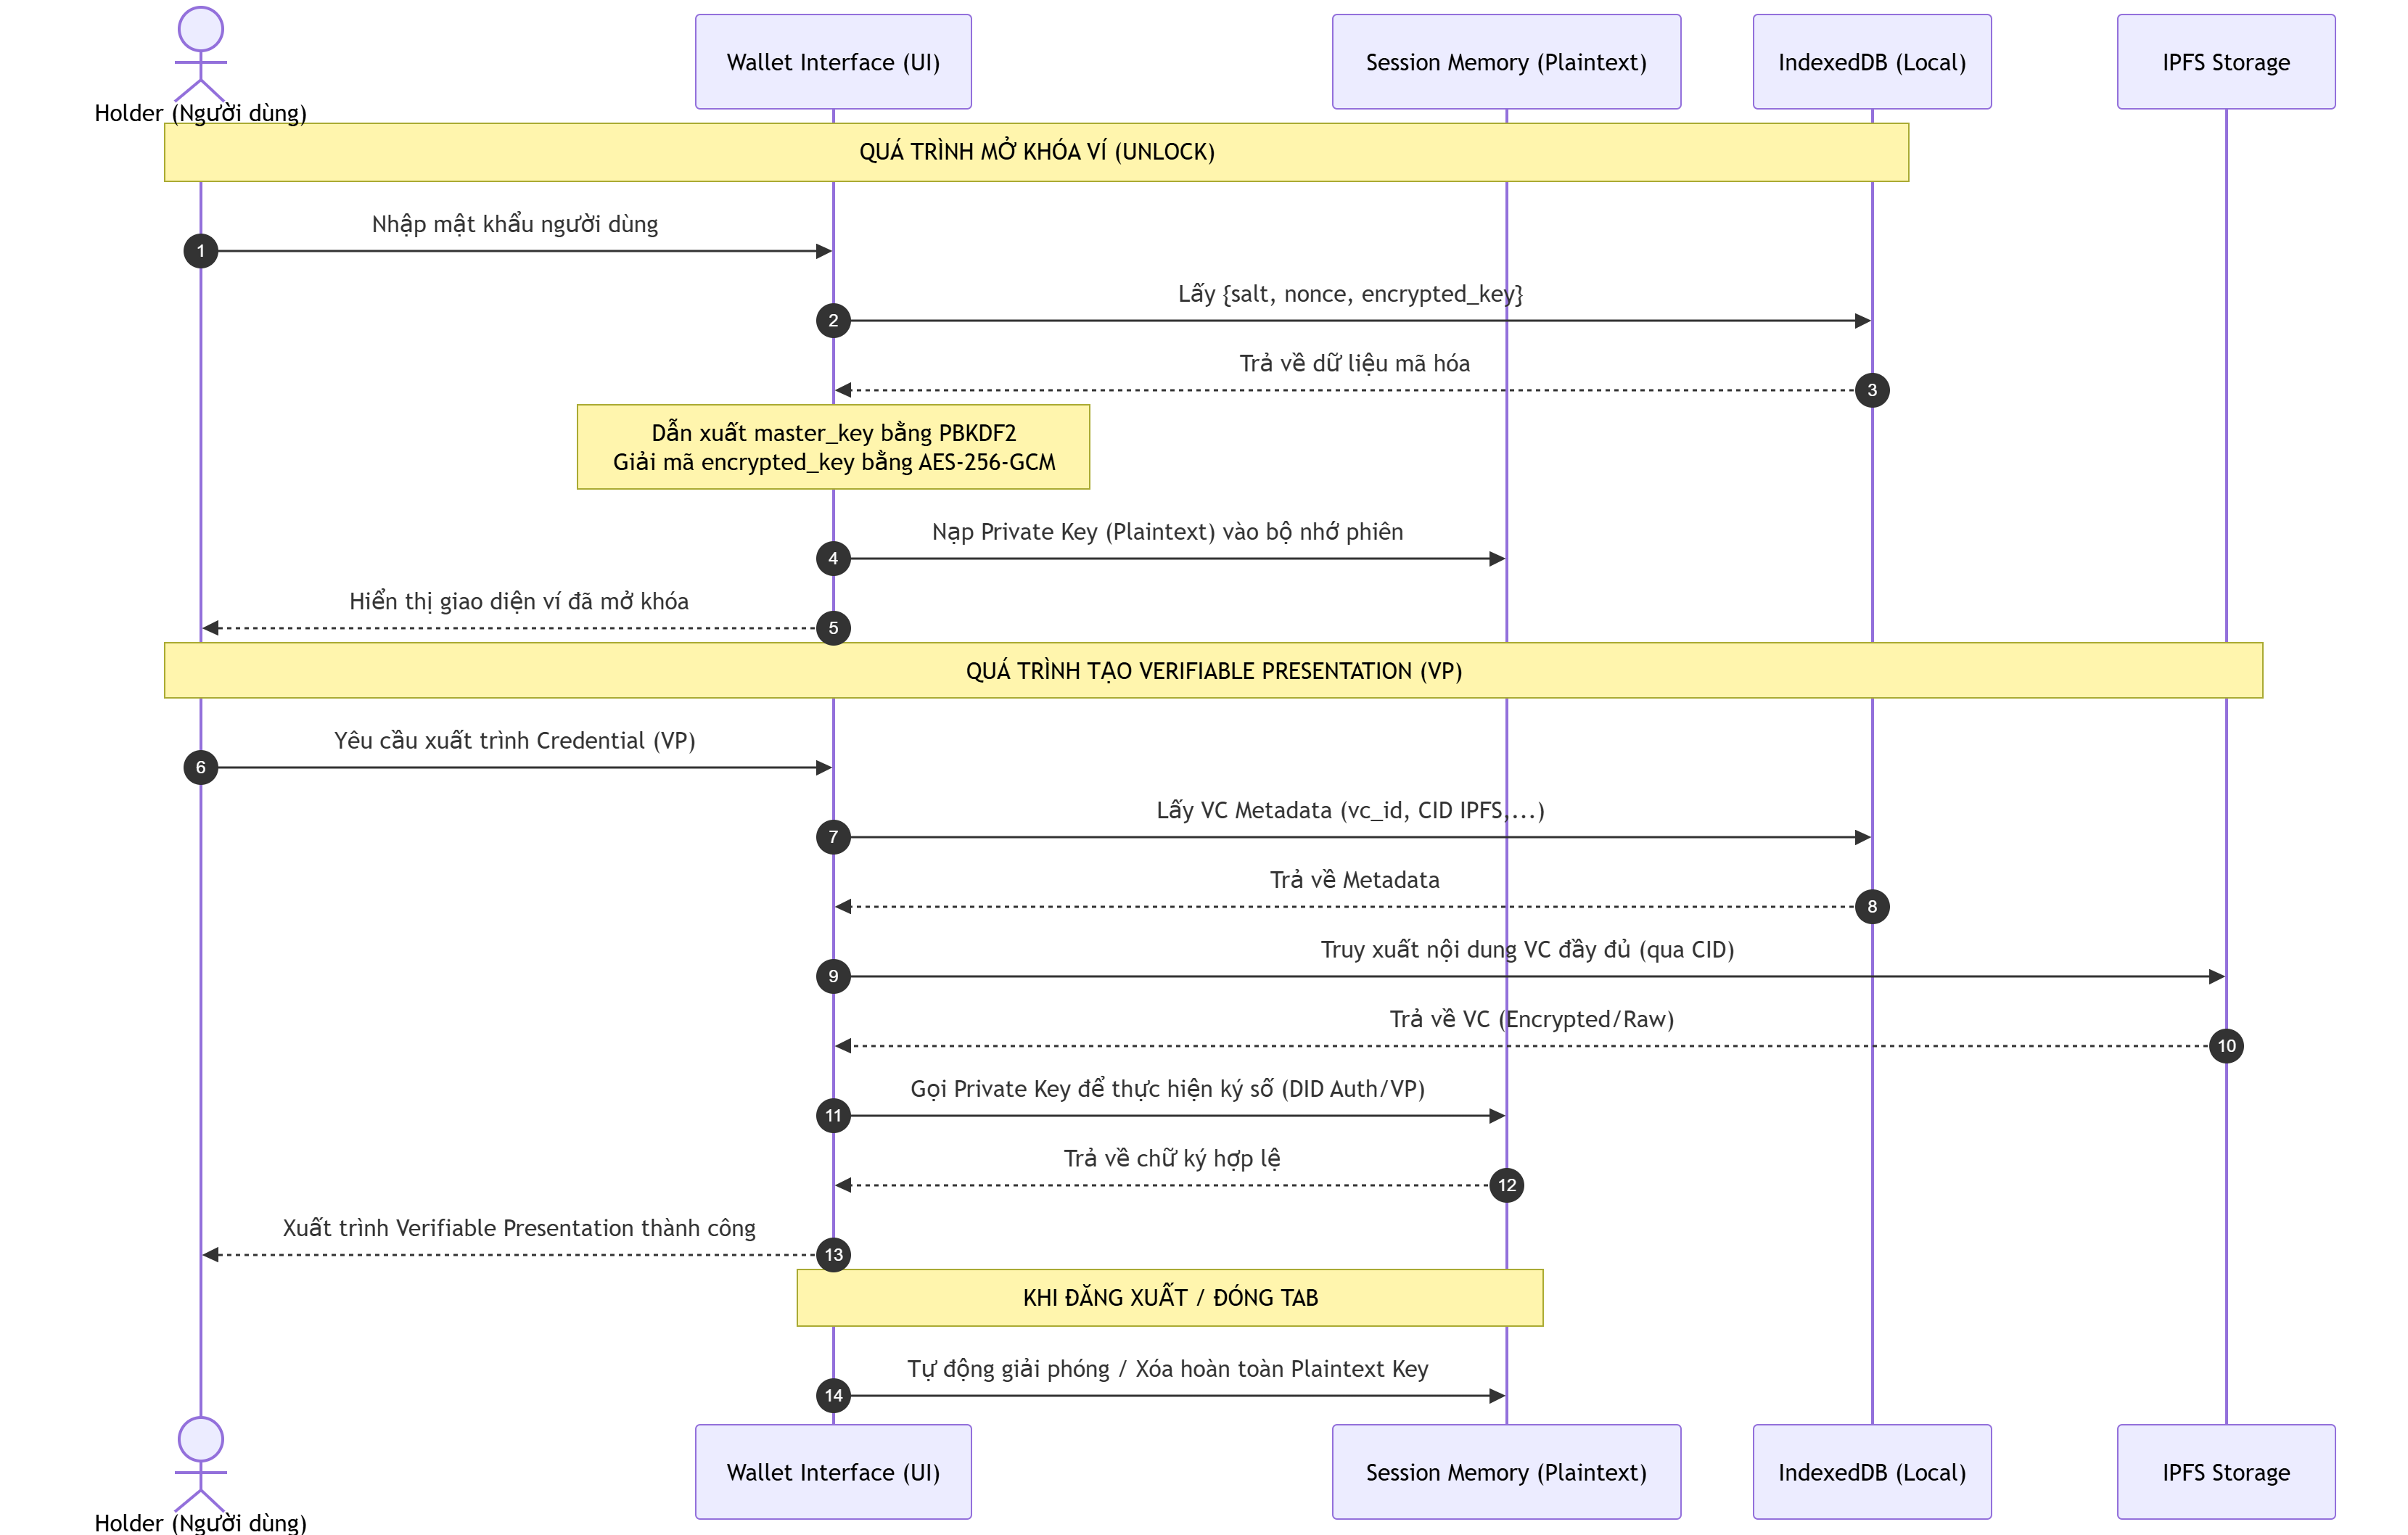
\includegraphics[width=0.92\textwidth]{images/mo-khoa-su-dung.png}
    \caption{Sơ đồ tuần tự mở khoá ví và dựng bản trình bày}
    \label{fig:v2-unlock}
\end{figure}

Để dùng trên thiết bị khác, khoá được dẫn xuất từ mười hai từ BIP-39 qua SLIP-0010 theo đường dẫn \texttt{m/44'/637'/0'/0'/0'}, trùng với đường dẫn của các ví phổ thông trong hệ sinh thái Move. Kết quả dẫn xuất đã được đối chiếu với bộ công cụ chính thức trên năm cụm từ ngẫu nhiên, khớp tuyệt đối ở cả khoá riêng, khoá công khai và địa chỉ. Giá trị kỳ vọng được lấy từ một nguồn độc lập chứ không do người viết kiểm thử tự đặt ra; nếu chỉ so với một hằng số tự nghĩ, phép kiểm sẽ đạt cả khi phép dẫn xuất sai.

\subsection{Tự ký và gửi giao dịch}

Phiên bản đầu của giao diện có ô ``Mã giao dịch'' ở mọi biểu mẫu: người dùng phải mở một ví ngoài, tự gọi hàm hợp đồng, chép mã giao dịch rồi dán lại. Thiết kế này sai ở hai mức. Về trải nghiệm, nó đẩy phần khó nhất sang người dùng trong khi trình duyệt đã có sẵn khoá. Về dữ liệu, giao diện không tự gửi giao dịch nên cũng không đọc được phản hồi. Số hiệu chứng thực do hợp đồng cấp nằm trong sự kiện \texttt{VCIssuedEvent} mà giao dịch phát ra, và vì không đọc được sự kiện đó, trường số hiệu trên chuỗi bị ghi cứng bằng không. Một trường bịa nằm im trong cơ sở dữ liệu, trông như dữ liệu thật.

Cách hiển nhiên là nhúng bộ công cụ của nền tảng, nhưng điều đó đưa gói giao diện lên 4,98\,MB. Hướng đã chọn là nhờ chính nút đầy đủ tuần tự hoá giao dịch:

\begin{lstlisting}
POST /v1/transactions/encode_submission   <- giao dich chua ky
   -> chuoi thap luc phan cua thong diep can ky
ed25519.sign(thong diep, khoa rieng trong bo nho)
POST /v1/transactions                     <- giao dich + chu ky
GET  /v1/transactions/by_hash/{hash}      lap cho den khi xac nhan
\end{lstlisting}

Mã JavaScript của giao diện giảm xuống khoảng 410\,KB (khoảng 134\,KB sau nén gzip), đổi lại thêm một vòng gọi mạng mỗi giao dịch. Đường ký được kiểm chứng trên chuỗi thật bằng tuyến mô phỏng giao dịch, tuyến chạy đủ các bước giải mã tham số, tìm hàm, vào thân hàm và tính gas nhưng không ghi gì lên chuỗi. Quá trình này làm lộ ba chi tiết không có trong tài liệu: tham số kiểu dãy byte phải truyền dạng chuỗi thập lục phân chứ không phải mảng số; nút đầy đủ từ chối mô phỏng một giao dịch có chữ ký hợp lệ, nên phải gửi chữ ký toàn số không kèm khoá công khai thật; và khoá xác thực trong thông tin tài khoản là giá trị băm của khoá công khai chứ không phải bản thân khoá.

\section{Bảo mật nội dung văn bằng}
\label{sec:ma-hoa}

Ở bản báo cáo trước, nội dung văn bằng nằm dạng rõ trên IPFS và trong cơ sở dữ liệu của tầng dịch vụ: ai biết CID là đọc được họ tên, mã sinh viên và điểm. Yêu cầu được đặt ra là chỉ chủ thể, và những bên được chủ thể cho phép, đọc được nội dung, với mã hoá và giải mã chạy trên thiết bị.

Hệ thống dùng mã hoá lai. Mỗi văn bằng có một khoá nội dung ngẫu nhiên 256 bit, dùng cho AES-256-GCM với dữ liệu xác thực kèm theo là giá trị băm của định danh văn bằng; nhờ đó một bản mã không thể bị ghép sang một văn bằng khác. Khoá nội dung được bọc riêng cho từng người nhận theo lược đồ ECIES: khoá X25519 của người nhận được dẫn xuất từ khoá Ed25519 vốn đã có trong ví, một khoá X25519 tạm sinh cho mỗi lần bọc, rồi HKDF-SHA256 tạo khoá bọc. Vì khoá công khai Ed25519 của mọi thực thể đã nằm trong danh bạ công khai, bên phát hành mã hoá cho chủ thể mà không cần chủ thể trực tuyến. Thứ duy nhất được ghim lên IPFS là phong bì sau:

\begin{lstlisting}
{ "v": 1, "alg": "A256GCM",
  "aad": "vnu-vc:<gia tri bam dinh danh van bang>",
  "iv": "<12 byte>", "ct": "<ban ma noi dung>",
  "recipients": [
    { "kid": "<dia chi chu the>",     "role": "holder", "epk": "...", "iv": "...", "wk": "..." },
    { "kid": "<dia chi ben phat hanh>", "role": "issuer", "epk": "...", "iv": "...", "wk": "..." } ] }
\end{lstlisting}

Người nhận gồm chủ thể và bên phát hành; bên phát hành cần đọc lại để đối soát và cấp lại. Hệ thống cố ý \emph{không} có khoá lưu giữ của nhà trường: một khoá như vậy giúp khôi phục khi cả chủ thể lẫn bên phát hành mất khoá, nhưng người giữ nó đọc được mọi văn bằng, và lộ nó là lộ toàn bộ nội dung.

\textit{Giá trị băm trên chuỗi vẫn là của nội dung rõ.} Nhờ vậy bước kiểm toàn vẹn khi xác minh và bất biến về tuần tự hoá tất định không đổi. Nội dung rõ chứa định danh văn bằng ngẫu nhiên 122 bit nên giá trị băm này không dò ngược được với kẻ chỉ đọc chuỗi, đúng như thí nghiệm B. Hệ quả là tầng dịch vụ không còn thấy nội dung, nên không tính lại được giá trị băm lúc cấp như trước. Ba rào thay thế: tầng dịch vụ kiểm cấu trúc phong bì (đúng sáu trường, gắn với đúng văn bằng, có đúng chủ thể và bên phát hành là người nhận, từ chối mọi trường lạ để không ai nhét được bản rõ cạnh bản mã); ví của chủ thể tự đối chiếu nội dung vừa giải mã với giá trị băm trên chuỗi và báo ``văn bằng lỗi'' nếu lệch; và bước 6 khi xác minh. Thực ra rào cũ cũng chưa bao giờ chặn được một bên phát hành gian lận, vì chính bên đó neo giá trị băm.

\textit{Chia sẻ cho bên xác minh.} Chủ thể giải mã trên máy, dựng bản trình bày, rồi mã hoá bản trình bày bằng một khoá ngẫu nhiên đặt trong phần \emph{fragment} của liên kết, phần sau dấu \texttt{\#}. Trình duyệt không bao giờ gửi phần này lên máy chủ, nên máy chủ và IPFS chỉ giữ bản mã. Trình duyệt của bên xác minh giải mã rồi gửi bản rõ cho tầng dịch vụ để chạy bảy bước; tầng dịch vụ không lưu bản rõ, chỉ lưu báo cáo. Cách khác là chạy cả bảy bước trong trình duyệt để máy chủ không bao giờ thấy bản rõ. Cách đó bị loại vì nó tạo ra một cài đặt thứ ba của quy trình xác minh phải giữ khớp với hai cài đặt tầng dịch vụ. Giới hạn đã chấp nhận là bản rõ có mặt trong bộ nhớ máy chủ đúng lúc xác minh. Thu hồi liên kết thì máy chủ ngừng trả bản mã.

Mã hoá cho hai người nhận cộng giải mã một văn bằng điển hình mất trung vị 7,6\,ms và phân vị 95 là 13\,ms, đo trên Node.js với cùng thư viện giao diện dùng; mỗi văn bằng không phải chạy lại PBKDF2. Rủi ro mới đáng kể nhất thuộc về người dùng: mất khoá ví nay đồng nghĩa với mất khả năng tự đọc văn bằng của mình, chứ không chỉ mất quyền ký.

\section{Giao diện theo vai trò}
\label{sec:giao-dien}

Mỗi màn hình chỉ hiện những thao tác mà vai trò đó thật sự được phép làm trên chuỗi. Điều này không thay việc kiểm quyền, vì rào chắn thật vẫn ở hợp đồng, nhưng tránh để người dùng làm một thao tác chắc chắn thất bại. Các quy tắc được lấy thẳng từ Bảng \ref{tab:v2-role}: ô cấp bit uỷ quyền bị khoá nếu người dùng không phải gốc; thao tác cấp quyền quản trị viên và đề cử gốc chỉ có ở màn hình quản trị gốc; thẻ ký nhận quyền gốc nằm ở trang cá nhân vì lúc ký người đó chưa phải gốc; nút kích hoạt lại chứng thực chỉ có ở màn hình quản trị viên.

Mỗi thao tác ghi hiển thị năm bước: chuẩn bị dữ liệu, bảo đảm có gas, ký, chờ chuỗi xác nhận, ghi chỉ mục. Mã giao dịch hiện ra như \emph{kết quả}, kèm liên kết tới trình xem giao dịch. Việc tách bước có giá trị chẩn đoán: ba nguyên nhân thất bại thường gặp (thiếu gas, bị hợp đồng từ chối vì thiếu quyền, chuỗi xác nhận chậm) cần ba cách xử lý khác nhau. Thẻ gas cho phép mọi vai trò xin token thử nghiệm cho chính tài khoản của mình, vì đăng ký định danh cũng tốn gas. Hệ thống không có chức năng chuyển token nào.

\section{Các kịch bản sử dụng}
\label{sec:kich-ban}

Bảy kịch bản ở Bảng \ref{tab:v2-scenarios} bao phủ vòng đời văn bằng cùng các luồng quản trị, và là căn cứ cho bộ kiểm thử luồng nghiệp vụ ở Chương \ref{chap:danh-gia}. Mỗi kịch bản ghi rõ ai là người ký, vì trong kiến trúc này người ký giao dịch chính là căn cứ phân quyền: hợp đồng không tin bất kỳ tham số nào khai ``tôi là ai''.

\begin{longtable}{|c|p{2.6cm}|p{2.3cm}|p{4.5cm}|p{3.4cm}|}
\caption{Bảy kịch bản sử dụng bao phủ vòng đời văn bằng}
\label{tab:v2-scenarios} \\
\hline
\textbf{KB} & \textbf{Kịch bản} & \textbf{Người ký} & \textbf{Hàm hợp đồng và kiểm tra chính} & \textbf{Kết quả mong đợi} \\ \hline
\endfirsthead
\hline
\textbf{KB} & \textbf{Kịch bản} & \textbf{Người ký} & \textbf{Hàm hợp đồng và kiểm tra chính} & \textbf{Kết quả mong đợi} \\ \hline
\endhead
1 & Đăng ký định danh & Chủ thể & \texttt{register\_did}; định danh duy nhất, CID đúng độ dài, băm khớp nội dung & DID phân giải được, kiểm toàn vẹn đạt \\ \hline
2 & Phê duyệt bên phát hành & Gốc hoặc quản trị viên & \texttt{approve\_issuer}; bên được duyệt có định danh hoạt động; bit uỷ quyền chỉ gốc cấp & Bản ghi thẩm quyền có phạm vi, thời hạn \\ \hline
3 & Cấp phát chứng thực & Bên phát hành & \texttt{issue\_vc}; thẩm quyền còn hiệu lực, loại trong phạm vi, hai định danh hoạt động & Số hiệu đọc từ \texttt{VCIssuedEvent} \\ \hline
4 & Trình bày và xác minh & Chủ thể ký VP & Bảy bước ở Mục \ref{sec:xac-minh} & Hợp lệ, báo cáo từng bước \\ \hline
5 & Thu hồi thẩm quyền & Gốc hoặc quản trị viên & Đổi trạng thái bản ghi thẩm quyền & Chứng thực của đơn vị trượt bước 7 \\ \hline
6 & Thu hồi chứng thực & Bên đã cấp & \texttt{revoke\_vc}; chỉ cần quyền sở hữu & Chứng thực trượt bước 5, kể cả khi đơn vị đã hết hạn uỷ quyền \\ \hline
7 & Xác minh thất bại & --- & Sửa nội dung, đổi người trình bày, thu hồi & Báo đúng bước hỏng và đúng nguyên nhân \\ \hline
\end{longtable}


Hai kịch bản đầu đáng được mô tả kỹ hơn vì chúng chứa những chi tiết dễ làm sai. Ở kịch bản đăng ký định danh (Hình \ref{fig:v2-seq-did}), thứ tự các bước có ý nghĩa: DID Document phải được ghim lên IPFS \emph{trước} để có CID, rồi giá trị băm được tính trên đúng bản tuần tự hoá tất định của tài liệu, rồi mới ký giao dịch. Nếu băm trên một bản tuần tự hoá khác, chẳng hạn bản có khoảng trắng do thư viện in đẹp chèn vào, bước kiểm toàn vẹn khi phân giải sẽ hỏng dù dữ liệu nguyên vẹn. Tầng dịch vụ tính lại giá trị băm từ nội dung trước khi ghi chỉ mục chứ không tin giá trị máy khách gửi lên; điều này làm được vì DID Document công khai theo thiết kế, khác với nội dung văn bằng.

\begin{figure}[H]
    \centering
    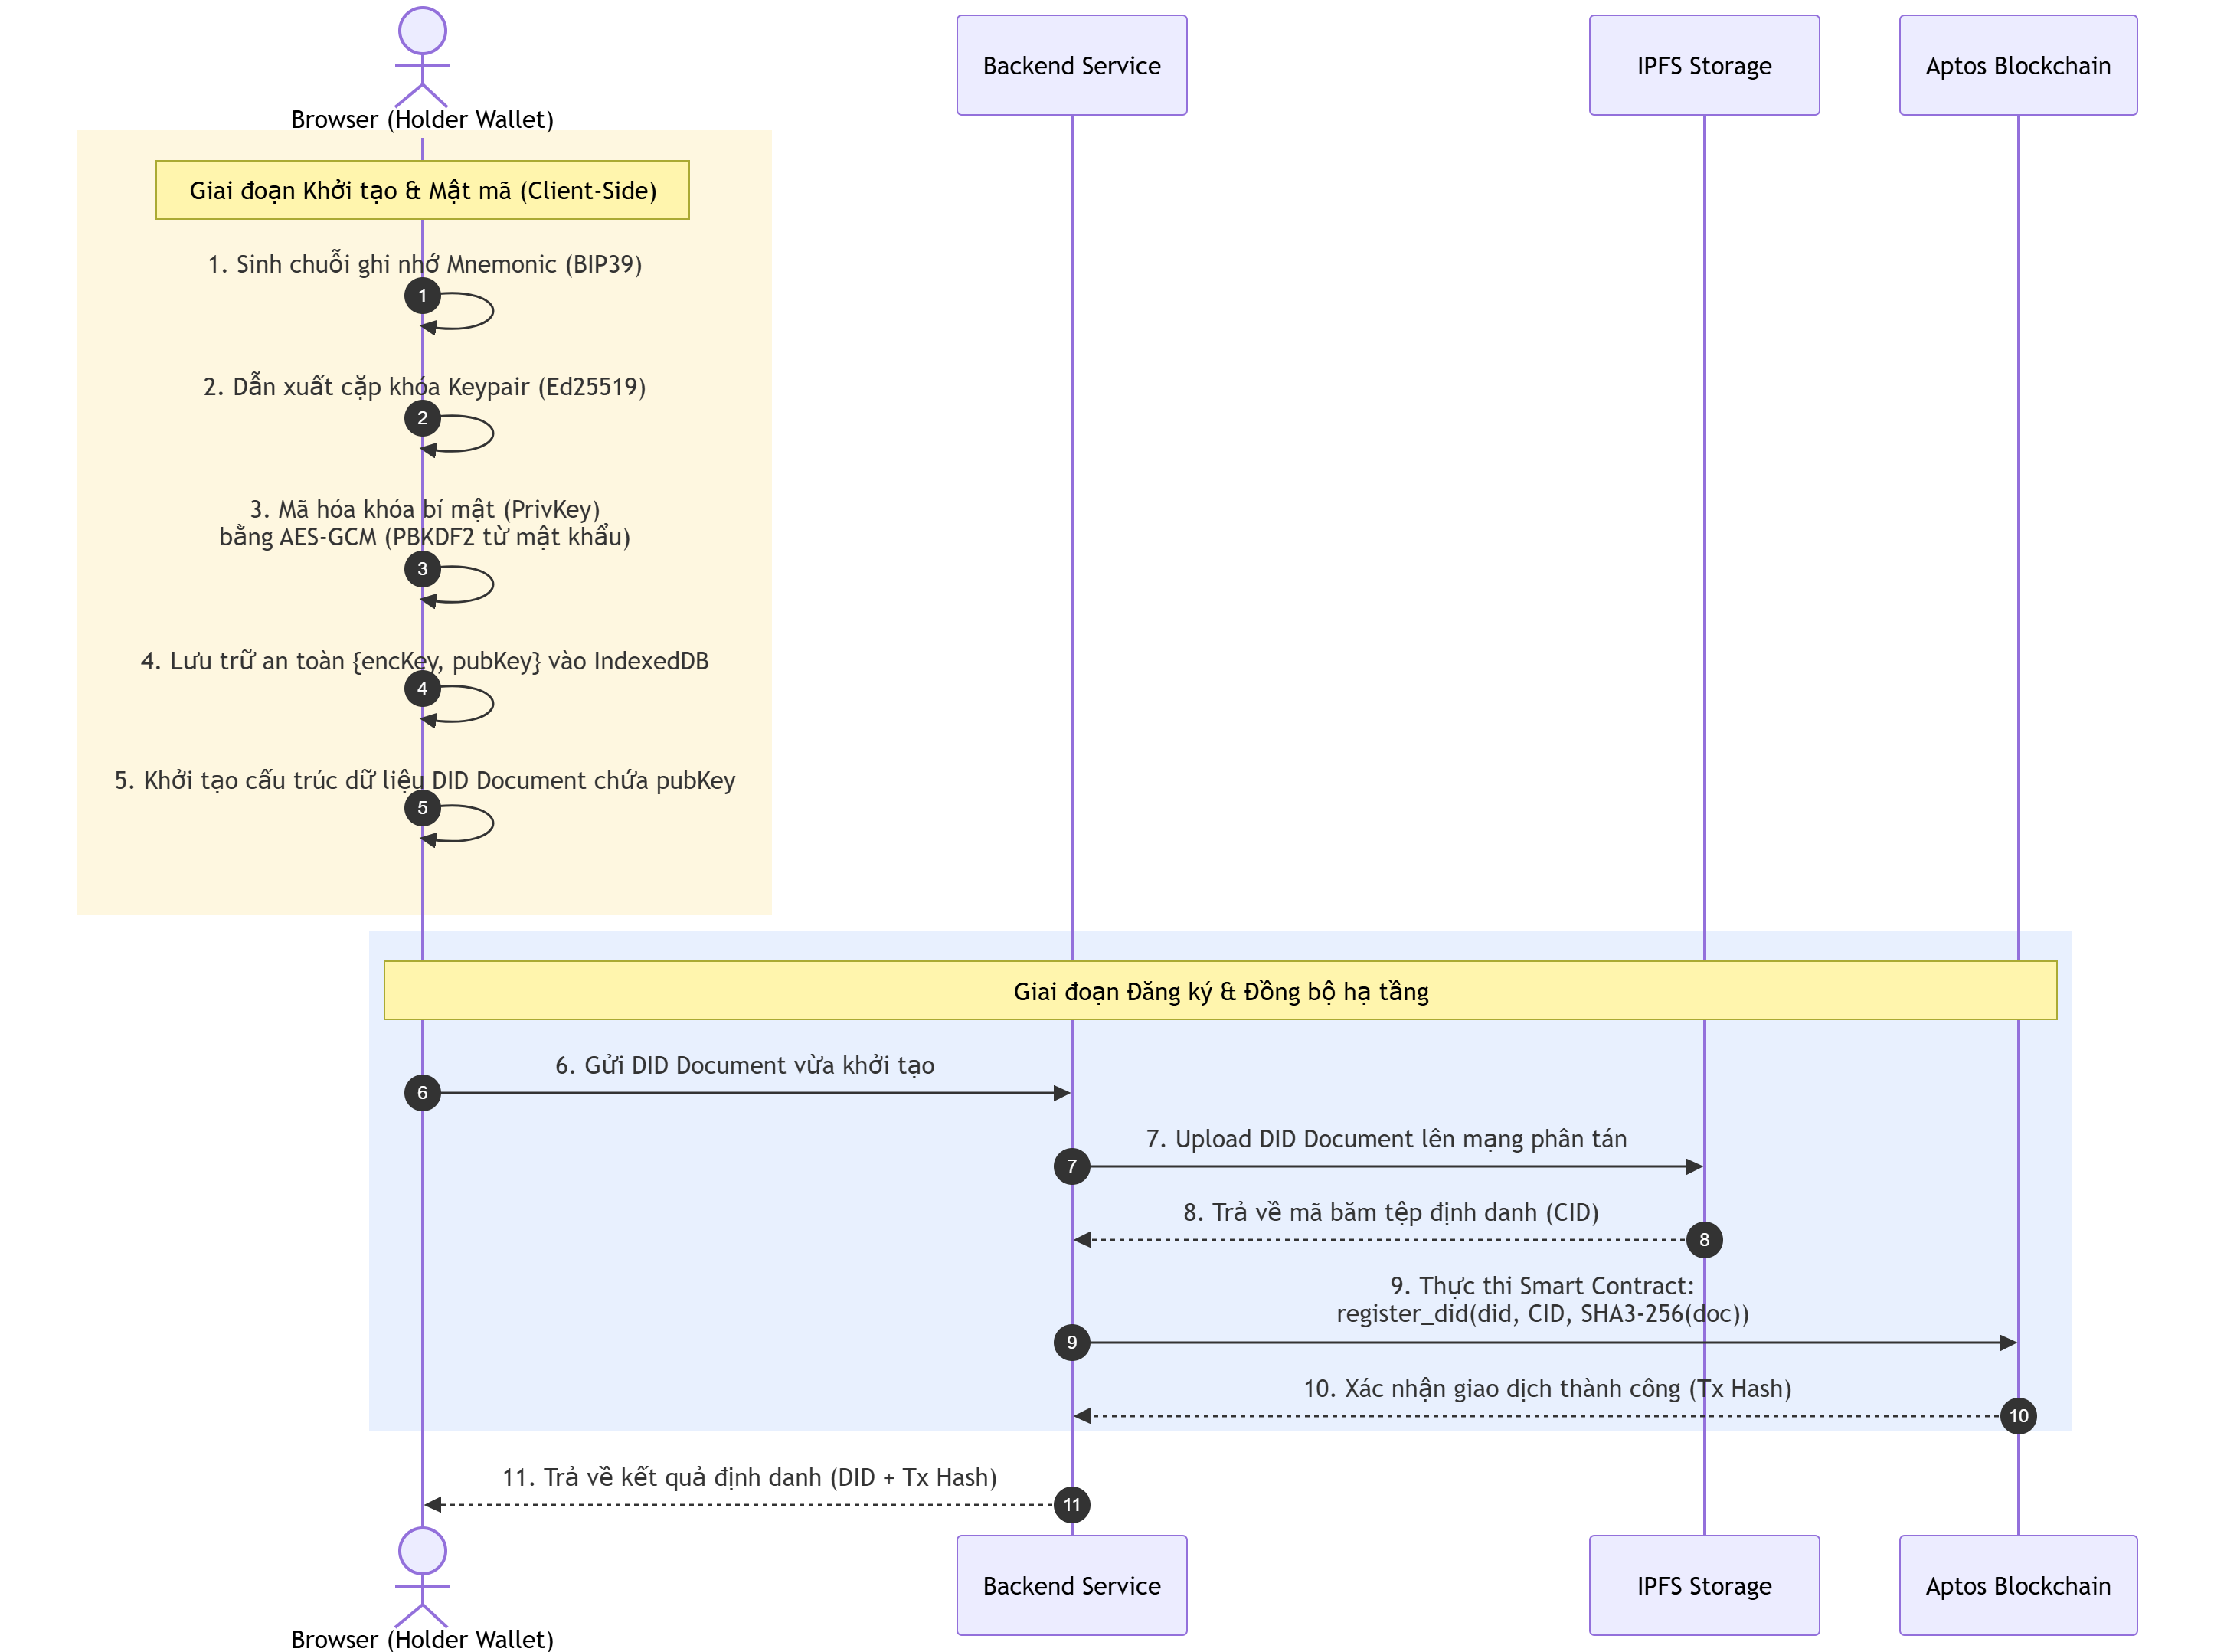
\includegraphics[width=0.95\textwidth]{images/seq_dang_ky_did_client.png}
    \caption{Sơ đồ tuần tự đăng ký định danh phía máy khách}
    \label{fig:v2-seq-did}
\end{figure}

Ở kịch bản cấp phát (Hình \ref{fig:v2-seq-issue}), số hiệu chứng thực trên chuỗi được đọc từ sự kiện \texttt{VCIssuedEvent} trong phản hồi của giao dịch rồi mới gửi cho tầng dịch vụ, thay vì để trống hay tự đánh số. Số hiệu này là thứ quản trị viên cần khi ký thao tác thu hồi; nếu phải gõ tay, gõ nhầm một chữ số là thu hồi nhầm văn bằng của người khác. Vì vậy tầng dịch vụ có tuyến trả về số hiệu trên chuỗi theo định danh chứng thực, và màn hình quản trị đọc số hiệu qua tuyến này. Số hiệu bắt đầu từ không: giao diện từng coi số không là ``chưa có số hiệu'', nên văn bằng đầu tiên của một gói mới sẽ không thu hồi được từ giao diện. Lỗi này được phát hiện khi gói trên chuỗi còn rỗng. Ở kịch bản này, nội dung văn bằng được mã hoá trước khi ghim (Mục \ref{sec:ma-hoa}), nên tầng dịch vụ chỉ kiểm cấu trúc phong bì chứ không kiểm lại giá trị băm nội dung.

\section{Khôi phục khi mất hoặc lộ khoá}
\label{sec:khoi-phuc}

Dữ liệu của người dùng nằm ở chỉ mục, IPFS và trên chuỗi, đều gắn với địa chỉ ví; thứ duy nhất không thay thế được nằm trên thiết bị là khoá riêng. Còn mười hai từ hoặc tệp sao lưu thì khôi phục được trên bất kỳ máy nào. Hai trường hợp còn lại được xử lý như sau.

\textit{Lộ khoá.} Chủ thể tự đình chỉ định danh của mình ngay trên giao diện. Mọi vai trò của địa chỉ ngừng ngay và không ai cấp được văn bằng mới cho nó. Tự đình chỉ thì tự mở lại được; nếu kẻ trộm khoá nhanh tay mở lại, quản trị viên đình chỉ đè và từ đó chỉ quản trị viên mở được.

\textit{Mất hết khoá.} Người dùng lập ví mới và đăng ký định danh mới. Quản trị viên đình chỉ hoặc thu hồi định danh cũ, xác minh danh tính ngoài hệ thống, rồi ghi nhận liên kết ví cũ--ví mới. Bên phát hành, vốn là một người nhận của phong bì, giải mã văn bằng cũ và cấp lại sang ví mới bằng hàm cấp lại; liên kết cũ--mới nằm trên chuỗi. Không có khoá lưu giữ nên nếu cả chủ thể lẫn bên phát hành cùng mất khoá, nội dung không khôi phục được từ hệ thống. Vì vậy giao diện nhắc sao lưu khi ví chưa có cách khôi phục nào trên máy, và nhắc kiểm tra lại mười hai từ sau 90 ngày: người dùng gõ lại đủ mười hai từ, ví dẫn xuất địa chỉ và so với ví đang mở, mà không cần lưu bí mật nào để kiểm. Sao lưu mã hoá bằng passkey là một hướng mở rộng (Mục \ref{sec:huong-phat-trien}).

\begin{figure}[H]
    \centering
    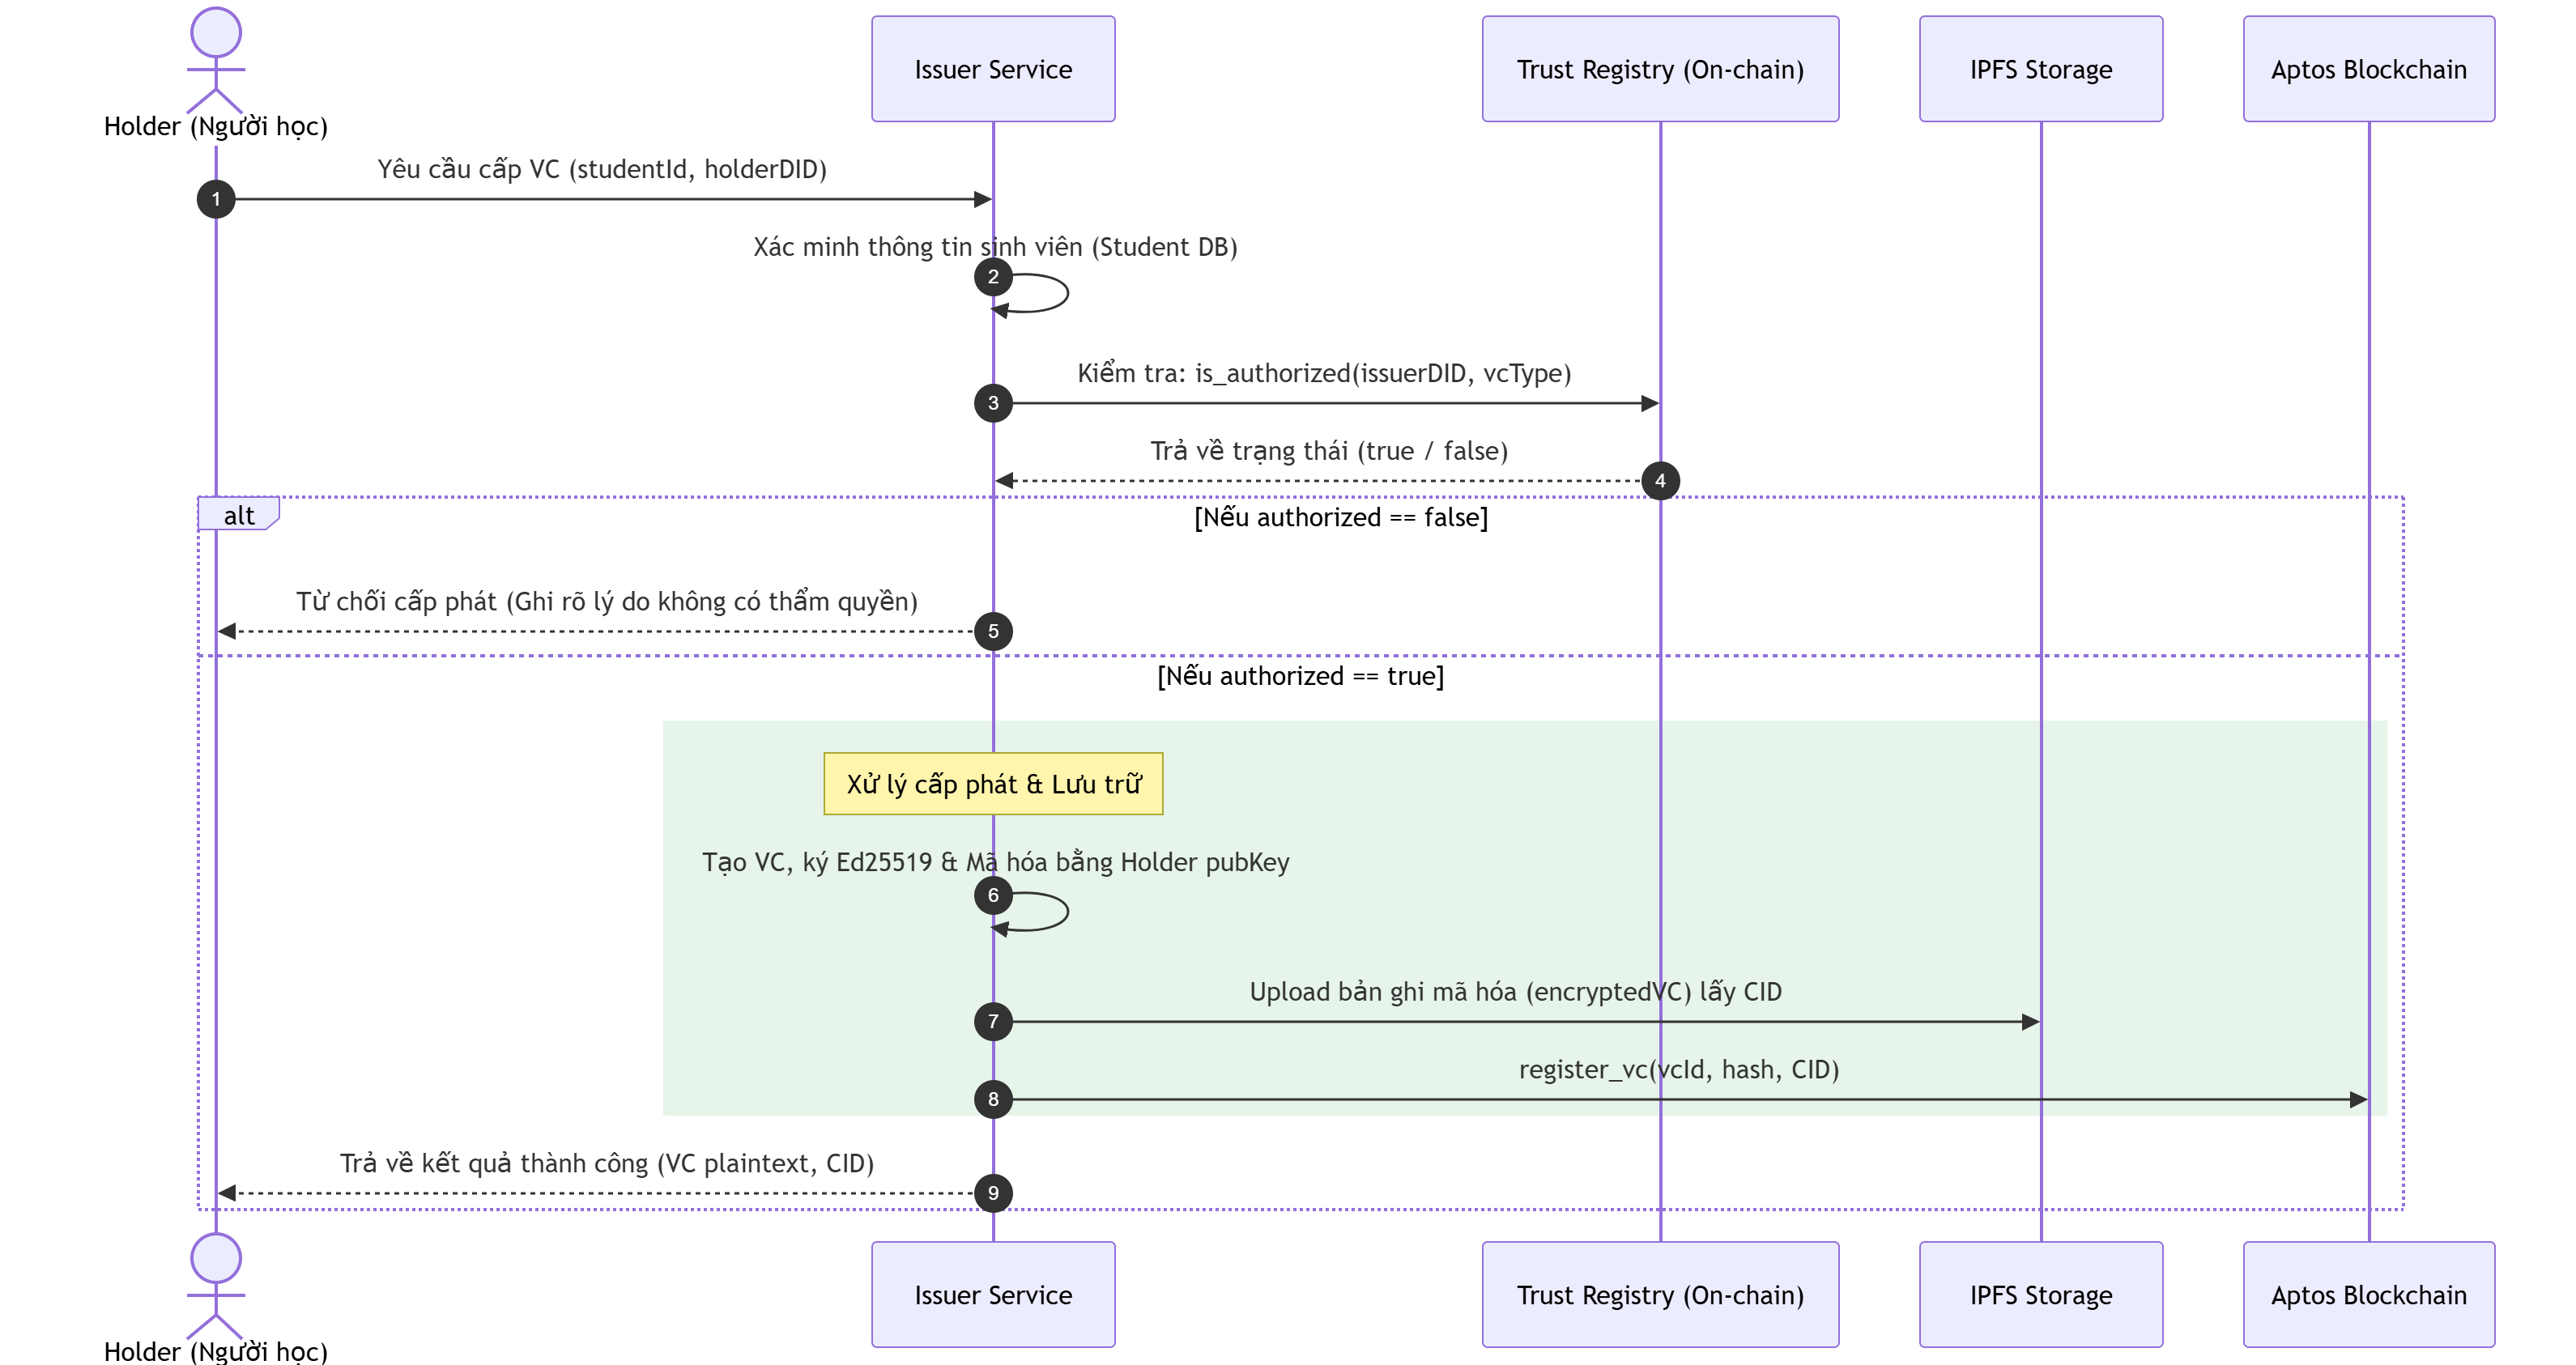
\includegraphics[width=0.95\textwidth]{images/seq_cap_phat_vc_authorized.png}
    \caption{Sơ đồ tuần tự cấp phát chứng thực}
    \label{fig:v2-seq-issue}
\end{figure}
